% $Id$

The NUOPC generic components are implemented as a {\em collection} of Fortran modules. Each module implements a single, well specified set of standard {\tt ESMF\_GridComp} or {\tt ESMF\_CplComp} methods. The nomenclature of the generic component modules starts with the {\tt NUOPC\_} prefix and continues with the flavor: {\tt Driver}, {\tt Model}, {\tt Mediator}, or {\tt Connector}. This is optionally followed by a string of additional descriptive terms. The four flavors of generic components implemented by the NUOPC Layer are:

\begin{itemize}

\item {\tt NUOPC\_Driver} - A generic driver component. It implements a child component harness, made of State and Component objects, that follows the NUOPC Common Model Architecture. It is specialized by plugging {\tt Model}, {\tt Mediator}, and {\tt Connector} components into the harness. {\tt Driver} components can be plugged into the harness to construct component hierarchies. The generic {\tt Driver} initializes its child components according to a standard Initialization Phase Definition, and drives their Run() methods according a customizable run sequence.

\item {\tt NUOPC\_Model} - A generic model component that wraps a model code so it is suitable to be plugged into a generic {\tt Driver} component.

\item {\tt NUOPC\_Mediator} - A generic mediator component that wraps custom coupling code (flux calculations, averaging, etc.) so it is suitable to be plugged into a generic {\tt Driver} component.

\item {\tt NUOPC\_Connector} - A generic component that implements Field matching based on metadata and executes simple transforms (Regrid and Redist). It can be plugged into a generic {\tt Driver} component.

\end{itemize}

The user code accesses the desired generic component(s) by including a {\tt use} line for each one. Each generic component defines a small set of public names that are made available to the user code through the {\tt use} statement. At a minimum the {\tt SetServices} method is made public. Some of the generic components define additional public routines and labels as part of their user interface. It is recommended to rename the entries of an imported generic component module in the local scope as part of the {\tt use} association. This prevents name clashes.

\begin{verbatim}
  use NUOPC_<GenericComp>, only: &
    <GenericComp>_SS      => SetServices, &
    <GenericComp>_labelA  => labelA
\end{verbatim}

A generic component is used by user code to implement a specialized version of the generic component. The user component derives from the generic component code by implementing its own public {\tt SetServices} routine that calls into the generic {\tt SetServices} routine before doing anything else. It is through this mechanism that the deriving component {\em inherits} from the generic component. The example shows how a specific model component is implemented to derive from the generic {\tt NUOPC\_Model}:

\begin{verbatim}
  use NUOPC_Model, only: &
    model_SS => SetServices

  subroutine SetServices(model, rc)
    type(ESMF_GridComp)  :: model
    integer, intent(out) :: rc

    ! derive this specific "model" component from generic NUOPC_Model
    call NUOPC_CompDerive(model, model_SS, rc=rc)

    ! specializing code for "model" to follow
    
  end subroutine
\end{verbatim}

There are three mechanisms through which user code specializes generic components. The first two methods specialize through call-back mechanisms into user implemented routines. The third method specializes by setting the values of parameters implemented by the generic component.

\begin{enumerate}

\item The specializing user code sets entry points for standard component methods not implemented by the generic component. Methods (and phases) that need to be implemented are clearly documented in the generic component description. The user code may further overwrite standard methods already implemented by the generic component code. However, this should rarely be necessary, and may indicate that there is a better fitting generic component available. Finally, some generic components come with generic routines that are suitable candidates for the standard component methods, yet require that the specializing code registers them as appropriate. Setting entry points for standard component methods is done in the {\tt SetServices} routine right after calling into the generic {\tt SetServices} method.

\item Some generic components require that specific methods are attached to the component. If a generic component uses specialization through attachable methods, the specific method labels (i.e. the names by which these methods are registered) and the purpose of the method are clearly documented. In some cases attachable methods are optional. This is clearly documented. Further, some generic components attach a default method to a label, which then is used for all phases. This default can be overwritten with a phase specific attachable method. Attaching methods to the component should be done in the {\tt SetServices} routine right after setting entry points for the standard component methods.

\item Some generic components offer methods that allow parameter specialization. The options of this specialization type are documentated as part of the {\tt Set()} methods.

\end{enumerate}

Components that inherit from a generic component may choose to only specialize certain aspects, leaving other aspects unspecified. This allows a hierarchy of generic components to be implemented with a high degree of code re-use. The variable level of specialization supports the very differing user needs. Figure \ref{fig:NUOPCGenericComp} depicts the inheritance structure of the standard generic components implemented by the NUOPC Layer. There are two trees, one is rooted in {\tt ESMF\_GridComp}, while the other is rooted in {\tt ESMF\_CplComp}.

\begin{figure}[h]
\begin{center}
\vspace{.5in}
\scalebox{0.6}{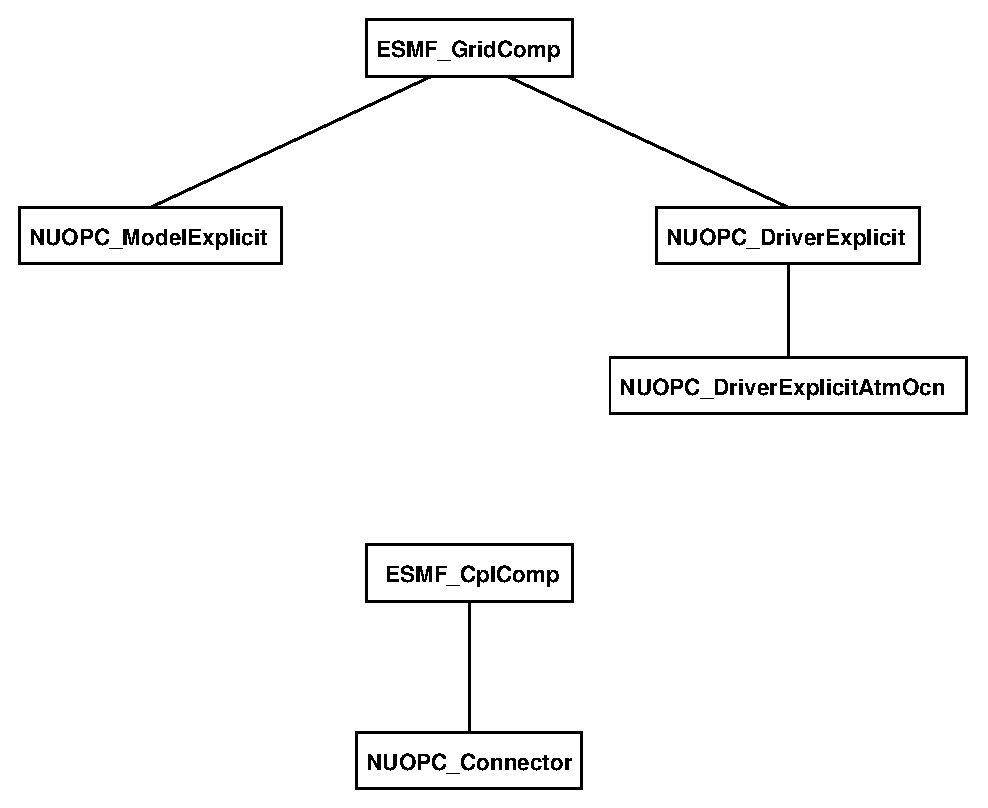
\includegraphics{NUOPC_GC}}
\end{center}
\caption{The NUOPC Generic Component inheritance structure. The tree on the left is rooted in {\tt ESMF\_GridComp}, while the tree on the right is rooted in {\tt ESMF\_CplComp}. The ESMF data types are shown in green. The four main NUOPC Generic Component flavors are shown in dark blue boxes. The yellow box shows a partial specialization in the inheritance tree.}
\label{fig:NUOPCGenericComp}
\end{figure}



